\documentclass[11pt]{article}

\usepackage{fontspec}
\usepackage[vietnamese]{babel}

\usepackage{graphicx}
\usepackage{amsmath, amssymb, amsfonts, bm}
\usepackage{xcolor}
\usepackage{hyperref}
\usepackage{pifont}
\newcommand{\xmark}{\ding{55}}
\newcommand{\cmark}{\ding{51}}
\usepackage{array}
\usepackage{float}
\usepackage{appendix}

\hypersetup{
    colorlinks=true,
    linkcolor=blue,
    filecolor=magenta,
    urlcolor=red,
    pdftitle={Overleaf Example},
    pdfpagemode=FullScreen,
}

\setmainfont{Times New Roman}
\setsansfont{Arial}
\setmonofont{Courier New}


% Page layout
\setlength{\topmargin}{-.5in}
\setlength{\textheight}{9.25in}
\setlength{\oddsidemargin}{0in}
\setlength{\textwidth}{6.8in}

% Title formatting
\usepackage{titling}
\setlength{\droptitle}{-10em}
\pretitle{%
    \begin{center}
    \LARGE\bfseries\textcolor{green}
    \end{center}
}
\posttitle{%
    \begin{center}
    \LARGE\bfseries\textcolor{cyan}
    \end{center}
}
\title{{Module Project}\\[0.5em]\textcolor{cyan}{RAG (Retrieval-Augmented Generation) sử dụng Streamlit}}
\author{Đinh Nhật Thành}
\date{}
\renewcommand{\maketitle}{}

% Fancy header/footer
\usepackage{fancyhdr}
\pagestyle{fancy}
\fancyhf{}
\renewcommand{\footrulewidth}{0.4pt}
\lhead{\bfseries AI VIETNAM}
\rhead{\bfseries aivietnam.edu.vn}
\fancyfoot[C]{\thepage}

% Section format (không đánh số section)
\usepackage{titlesec}
\titleformat{\section}
{\normalfont\Large\bfseries}
{}{0em}{}

% Listings (code block)
\usepackage{listings}
\definecolor{codegreen}{rgb}{0,0.6,0}
\definecolor{codegray}{rgb}{0.5,0.5,0.5}
\definecolor{codepurple}{rgb}{0.58,0,0.82}
\definecolor{backcolour}{rgb}{0.95,0.95,0.92}
\lstdefinestyle{mystyle}{
    backgroundcolor=\color{backcolour},
    commentstyle=\color{codegreen},
    keywordstyle=\color{magenta},
    numberstyle=\tiny\color{codegray},
    stringstyle=\color{codepurple},
    basicstyle=\ttfamily\footnotesize,
    breaklines=true,
    captionpos=b,
    keepspaces=true,
    numbers=left,
    numbersep=5pt,
    tabsize=2,
    showspaces=false,
    showstringspaces=false,
    showtabs=false
}
\lstset{style=mystyle}

% Colored boxes
\usepackage[many]{tcolorbox}
\definecolor{sub}{HTML}{cde4ff}
\newtcolorbox{boxC}{
    colback = sub,
    boxrule = 0pt
}

% For math proofs or custom counters (tuỳ chọn nếu cần)
\usepackage{lipsum}
\newcounter{mycounter}
\newcommand\showmycounter{\stepcounter{mycounter}\themycounter}
\newcommand\showlips{\stepcounter{mycounter}\lipsum[\value{mycounter}]}

% Others
\usepackage{booktabs}
\usepackage{subcaption}
\usepackage{framed}
\usepackage{tikz}


%%%%%%%%%%%%%%%%%%%%%%%%%%%%%%%%%%%%%%%%%%%%%%%%%%%%%%%%%%%%%%%%%%%%%%%%%%%%%
%%%%%%%%%%%%%%%%%%%%%%%%%%%%%%%%%%%%%%%%%%%%%%%%%%%%%%%%%%%%%%%%%%%%%%%%%%%%%
%%%%%%%%%%%%%%%%%%%%%%%%%%%%%%%%%%%%%%%%%%%%%%%%%%%%%%%%%%%%%%%%%%%%%%%%%%%%%
\begin{document}
\maketitle

\begin{titlepage}
    \centering
    \vspace*{\fill}

    {\Huge \textbf{\thetitle} \par}
    \vspace{2em}

    {\Large \textbf{\theauthor} \par}
    \vspace{1em}

    {\large \today \par}

    \vspace*{\fill}
    \thispagestyle{fancy}
\end{titlepage}

\newpage
\tableofcontents
\thispagestyle{fancy}

%? Indentation for paragraphs
\setlength{\parindent}{2em} % hoặc giá trị Ta muốn, ví dụ 1.5em, 20pt, v.v.


%1%%%%%%%%%%%%%%%%%%%%%%%%%%%%%%%%%%%%%%%%%%%%%%%%%%%%%%%%%%%%%%%%%%%%%%%%%%%%%%%%%%%%%%%%%%%%%%%%%%%%%%%%%%%%%%%%%%%%%%%%%%%%%%%%%%%%%%%%%%%%%%%%%%%%%%%%%%%%%%%%%%%%%%%%%%%%%%%%%%%%%%%
\newpage

\renewcommand{\thesubsection}{\arabic{subsection}}
\newpage

% Link to Appendix (Phụ Lục)
\section{Giải thích thuật ngữ}
Khi trong bài có từ ngữ chuyên ngành khó hiểu, bạn có thể xem giải thích chi tiết một số thuật ngữ quan trọng dưới đây:

\begin{itemize}
    \item \textbf{Parse (Phân tích cú pháp):}
    Là quá trình chuyển chuỗi ký tự thành cấu trúc dữ liệu. \hyperref[app:parse]{Parse (Phụ lục)}

    \item \textbf{Protocol (Giao thức):}
    Tập hợp quy tắc giao tiếp giữa các hệ thống. \hyperref[app:protocol]{Protocol (Phụ lục)}

    \item \textbf{Synchronous vs. Asynchronous:}
    Liên quan đến thời điểm thực hiện tác vụ. \hyperref[app:synchronous_asynchronous]{Synchronous Asynchronous (Phụ lục)}
\end{itemize}


% Main Section
%? thêm lùi dòng 1em vào đầu mỗi đoạn văn bản trong phần này
\section{Mở Đầu}
\subsection{Mô tả bài toán}
Trong kỷ nguyên của mô hình ngôn ngữ lớn (LLM), việc xây dựng hệ thống hỏi–đáp thông minh từ tài liệu cá nhân hoặc doanh nghiệp đang trở nên phổ biến. Tuy nhiên, các LLM như GPT-4 hay Gemini vốn không có quyền truy cập trực tiếp vào tài liệu riêng lẻ (như notes học tập, báo cáo tuần, hợp đồng nội bộ, v.v.). Điều này dẫn đến nhu cầu xây dựng các hệ thống truy hồi kết hợp sinh (Retrieval-Augmented Generation – RAG), giúp LLM “nhớ” đúng những gì người dùng cung cấp.


\subsection{Nội dung bài viết}
Trong bài viết này, chúng ta xây dựng một Web App đơn giản, sử dụng \textbf{Streamlit}, 1 thư viện giúp xây dựng UI 1 cách nhanh chóng và mô hình \textbf{RAG}, 1 kỹ thuật xử lý ngôn ngữ cho phép người dùng hỏi đáp dựa trên nội dung từ các Notes (ví dụ: \texttt{M1W1\_Wednesday.pdf}) thuộc chương trình học \textbf{AIO Conquer 2025}. Các bước thực hiện bao gồm:
\begin{itemize}
    \item Người dùng tải tài liệu PDF lên giao diện \texttt{Streamlit}.
    \item Hệ thống sử dụng \texttt{PyPDFLoader} để phân tích nội dung văn bản.
    \item Văn bản được chia nhỏ thành các đoạn (chunk) khoảng 500 tokens bằng \texttt{SemanticChunker}.
    \item Mỗi đoạn được mã hoá thành vector bằng \texttt{HuggingFaceEmbeddings}, lưu trong vector DB \texttt{Chroma}.
    \item Khi người dùng đặt câu hỏi, hệ thống truy hồi các đoạn liên quan, kết hợp vào một prompt, rồi gửi đến LLM để sinh ra câu trả lời phù hợp theo ngữ cảnh.
\end{itemize}

\begin{figure}[H]
    \centering
    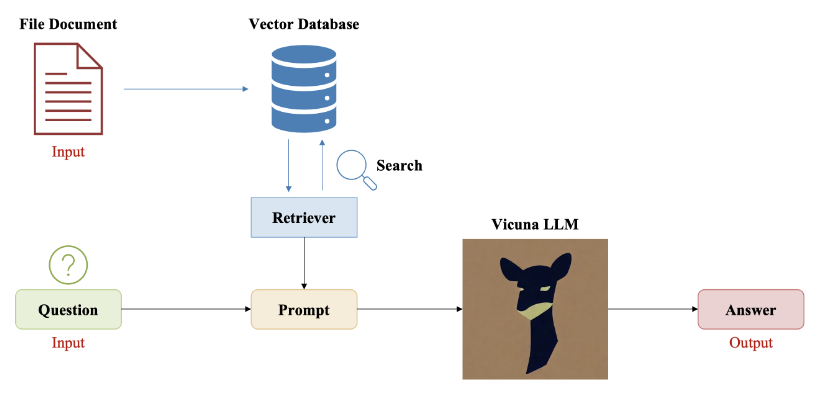
\includegraphics[width=0.85\textwidth]{architecture.png}
    \caption{Luồng dữ liệu và thành phần chính của ứng dụng RAG trên Streamlit}
\end{figure}

\vspace{0.5em}
\textbf{Nội dung bài viết} không chỉ dừng lại ở việc xây dựng ứng dụng, mà còn tập trung vào việc giải thích tổng quan mô hình RAG – các thành phần cốt lõi, những khó khăn khi xây dựng RAG bằng công cụ cơ bản, và vì sao cần một framework như LangChain để đơn giản hóa và chuẩn hóa quy trình.

\vspace{0.5em}
\textbf{Mục tiêu bài viết} là giúp người đọc – đặc biệt là người mới bắt đầu – tiếp cận RAG một cách căn bản, có hệ thống, dựa trên tư duy \textit{First Principle Thinking}: bắt đầu từ bài toán thực tế, xác định vấn đề tồn tại, rồi từng bước đi đến giải pháp tối ưu với LangChain.


\section{LangChain framework cho xây dựng hệ thống RAG}
\subsection{Các thành phần cốt lõi của RAG}
Để hiểu vì sao LangChain lại hữu ích trong việc xây dựng hệ thống RAG, trước tiên ta cần nắm rõ các thành phần cốt lõi của mô hình này.

\label{sec:rag_core}
\begin{itemize}
    \item \textbf{Retrieval} (Truy hồi): Sau khi người dùng hoàn tất việc tải tài liệu lên Vector Database và bắt đầu hỏi. RAG sẽ truy vấn các đoạn văn bản liên quan nhất tới câu hỏi sử dụng thông tin của văn bản được \hyperref[app:embedding]{Embedding} trong Vector Database.
    \item \textbf{Augmentation} (Tăng cường ngữ cảnh): Giúp mô hình LLM hiểu hơn về ngữ cảnh bằng cách kết hợp các đoạn text được truy hồi trong bước Retrieval, ví dụ đầu ra hoặc yêu cầu đi kèm người dùng muốn vào prompt.
    \item \textbf{Generation} (Sinh ngôn ngữ): Mô hình ngôn ngữ lớn (LLM) nhận prompt có kèm ngữ cảnh trong bước Augmentation và sinh ra câu trả lời.
\end{itemize}

\vspace{-0.5em}
\noindent
\textit{Tại sao dùng RAG?}
Cho phép câu trả lời được \textbf{dựa trên dữ liệu thực tế}, giảm \textbf{hallucination} và hỗ trợ \textbf{cập nhật thông tin mới} mà không cần fine-tuning lại toàn bộ mô hình. \\ \\

\textbf{Một hệ thống RAG cơ bản thường bao gồm:}
\begin{enumerate}
    \item \textbf{Text Loader:} trích xuất văn bản từ các nguồn như PDF, TXT, DOCX, v.v.
    \item \textbf{Text Splitter:} chia nhỏ văn bản thành các đoạn ngắn, không quá dài để phù hợp với giới hạn đầu vào của mô hình.
    \item \textbf{Embedding Model:} mã hóa mỗi đoạn thành vector bằng mô hình học máy (vd: \texttt{all-MiniLM}, \texttt{Instructor}, v.v.).
    \item \textbf{Vector Database:} lưu trữ các vector để có thể truy hồi nhanh những đoạn gần nhất với câu hỏi.
    \item \textbf{Retriever:} tìm các đoạn liên quan nhất dựa trên câu hỏi của người dùng.
    \item \textbf{Prompt + LLM:} ghép các đoạn được tìm thấy vào một mẫu prompt, rồi gửi đến mô hình ngôn ngữ để tạo câu trả lời.
\end{enumerate}

\vspace{1em}

\subsection{Vấn đề tồn tại khi xây dựng mô hình RAG (không dùng framework)}

Mặc dù ý tưởng của RAG khá đơn giản, nhưng nếu Ta là người mới và tự xây dựng hệ thống từ đầu, Ta sẽ gặp nhiều khó khăn. Dưới đây là các vấn đề phổ biến mà nhiều người mới gặp phải:

\begin{enumerate}
    \item \textbf{Thiếu chuẩn hóa quy trình:}
    \begin{itemize}
        \item Không có "hướng đi rõ ràng" nên dễ bị lạc giữa việc: nên xử lý văn bản trước hay làm embedding trước? Nên lưu vector ở đâu?
        \item Dễ viết code rời rạc, khó kiểm soát pipeline tổng thể.
    \end{itemize}

    \item \textbf{Lỗi khi kết nối các bước thủ công:}
    \begin{itemize}
        \item Mỗi bước (load → split → embed → lưu → truy vấn → prompt → gọi LLM) cần thư viện riêng.
        \item Ví dụ: dùng \texttt{PyPDF2} để load, \texttt{sentence\_transformers} để embed, \texttt{FAISS} để lưu vector → khó đồng bộ.
        \item Việc truyền dữ liệu giữa các bước cũng dễ bị lỗi do định dạng không đồng nhất.
    \end{itemize}

    \item \textbf{Viết prompt thủ công tốn thời gian:}
    \begin{itemize}
        \item Ta phải tự viết prompt để đảm bảo LLM hiểu ngữ cảnh, tránh trả lời ngoài lề.
        \item Khi tăng số đoạn truy hồi, prompt cũng phải được chỉnh lại — dễ gây lỗi hoặc rối logic.
    \end{itemize}

    \item \textbf{Khó mở rộng hoặc tái sử dụng pipeline:}
    \begin{itemize}
        \item Nếu Ta muốn thay thế embedding model, hoặc chuyển từ Chroma sang FAISS, Ta phải chỉnh lại nhiều đoạn code.
        \item Việc tái sử dụng workflow trong project khác gần như phải viết lại từ đầu.
    \end{itemize}

    \item \textbf{Không dễ chạy song song hoặc debug từng bước:}
    \begin{itemize}
        \item Ta không thể theo dõi đầu ra từng bước (ví dụ sau khi chunk, sau khi embed, sau khi truy hồi).
        \item Khi có lỗi (ví dụ truy hồi sai đoạn), khó biết nguyên nhân nằm ở bước nào.
    \end{itemize}
\end{enumerate}

\vspace{1em}

\subsection{Giải pháp mà LangChain đưa ra}
Một trong những điểm mạnh nổi bật của LangChain là việc xây dựng mỗi thành phần trong RAG thành một \textbf{Modular Component} – nghĩa là mỗi bước như:
\begin{itemize}
    \item Tải tài liệu (\texttt{DocumentLoader})
    \item Chia nhỏ văn bản (\texttt{TextSplitter})
    \item Mã hoá thành vector (\texttt{Embeddings})
    \item Lưu trữ/truy vấn (\texttt{VectorStore}, \texttt{Retriever})
    \item Khai báo LLM (\texttt{LLM})
    \item Tạo sinh câu trả lời sử dụng LLM (\texttt{LLMChain})
\end{itemize}
đều được đóng gói dưới dạng một \texttt{Class riêng biệt}. Điều này mang lại 3 lợi ích quan trọng:
\begin{itemize}
    \item \textbf{Tái sử dụng:} Dễ tái sử dụng từng thành phần trong nhiều ứng dụng khác nhau.
    \item \textbf{Kiểm thử dễ dàng:} Có thể test từng bước độc lập (vd: kiểm tra chỉ \texttt{TextSplitter} hoặc \texttt{Retriever}).
    \item \textbf{Thay thế linh hoạt:} Chỉ cần thay 1 class là có thể chuyển từ mô hình OpenAI sang HuggingFace hoặc thay FAISS bằng Chroma mà không ảnh hưởng toàn bộ hệ thống.
\end{itemize}

\vspace{1em}

\noindent
Ngoài ra LangChain đơn giản hóa và tối ưu quy trình xây dựng hệ thống bằng cách sử dụng 1 lớp xây dựng gọi là \textbf{Runnable: lớp bao bọc (wrapper)}
Thay vì chỉ viết các hàm thủ công như Python thông thường, LangChain sử dụng Object \texttt{Runnable} như một lớp bao (wrapper) giúp Ta:

\begin{itemize}
    \item Biến mọi thao tác (dù đơn giản như một hàm `lambda`) thành một “khối logic” có thể:
        \begin{itemize}
            \item chạy độc lập, (`RunnableLambda`)
            \item xâu chuỗi các hàm sử dụng RunnableSequence sử dụng ký hiệu (`|`), nó hoạt động tương tự như Pipe trong UnixLinux. (ví dụ: func1 | func 2)
            \item chạy song song (`RunnableMap`) cho phép xử lý các hàm 1 cách \textbf{đồng bộ (synchronous)} hoặc \textbf{bất đồng bộ (asynchronous)} mà Ta không cần viết thêm logic phức tạp.
        \end{itemize}

     \item Việc đối gộp các hàm như 1 khối logic, cho phép người phát triển tư duy theo luồng (pipeline) rõ ràng.
\end{itemize}

Khác với cách viết hàm truyền thống, \texttt{Runnable} giống như “\textit{block LEGO thông minh}”: dễ lắp, dễ thay, dễ mở rộng. Ngoài ra, Ta cũng có thể xem thêm phần giải thích về \hyperref[app:synchronous_asynchronous]{synchronous và asynchronous} trong phụ lục để hiểu rõ vì sao việc chuyển đổi giữa 2 kiểu thực thi này là quan trọng trong xây dựng ứng dụng quy mô lớn.

\vspace{0.5em}


Ví dụ:
\begin{lstlisting}[language=Python, caption=So sánh cách viết thường vs dùng Runnable trong LangChain]
# Hàm truyền thống
def upper(text):
    return text.upper()

# Hàm với LangChain Runnable
from langchain.schema.runnable import RunnableLambda

runnable_upper = RunnableLambda(lambda x: x.upper())
runnable_upper.invoke("langchain")  # Output: LANGCHAIN
\end{lstlisting}

Tuy đoạn code nhìn có vẻ dài hơn, nhưng khi ta muốn kết hợp nhiều bước thành pipeline, chạy đồng thời trên nhiều input, hoặc debugging từng bước giữa chain, thì hệ thống `Runnable` trở thành công cụ cực kỳ hữu ích và dễ mở rộng.

\vspace{1em}

\noindent
\textbf{Hỗ trợ sẵn hàng chục thư viện phổ biến:}
\begin{itemize}
	\item Ví dụ: Ta có thể dùng FAISS, Chroma, Weaviate,... chỉ với vài dòng code thay vì cấu hình thủ công.
	\item Tương tự với OpenAI, HuggingFace, Claude, v.v. \\
\end{itemize}


\noindent
\textbf{Tối ưu khả năng mở rộng:}
Ta có thể mở rộng từ một ứng dụng RAG đơn giản sang hệ thống đa tác nhân, phân nhánh, tích hợp phản hồi người dùng (feedback loop) mà không phải viết lại toàn bộ code. \\

\noindent
\textbf{Tích hợp dễ dàng với các framework UI như Streamlit, Gradio:}
Ta có thể kết nối backend LangChain với frontend dễ dàng qua API hoặc trực tiếp embed trong app Streamlit. \\

\noindent
\textbf{Tóm lại:} LangChain không phải là công cụ “thay thế” các thư viện cơ bản, mà là framework kết nối chúng theo một cách mạch lạc, mở rộng được, và giúp Ta tập trung vào logic thay vì xử lý từng bước nhỏ. Nhờ đó, chỉ với 5–10 dòng code Ta đã có được full RAG pipeline, dễ maintain và mở rộng thêm tính năng (chaining, branching, agents…).

% Tiếp theo là phần “Giải thích các syntax cơ bản…” sẽ làm sau nhé.
\subsection{Giải thích các syntax cơ bản của LangChain}
Trong LangChain, các \textbf{Runnable} là những khối xây dựng cơ bản, mỗi Runnable đại diện cho một tác vụ hoặc hoạt động đơn lẻ. Về bản chất, một Runnable là một đối tượng Python được thiết kế để tối ưu hóa hàm của Ta bằng cách sử dụng tính song song.

\subsubsection*{Khái niệm chính về Runnables trong LangChain}
\begin{itemize}
    \item \textbf{Tính mô đun (Modularity):}
    \begin{boxC}
        Mỗi \texttt{Runnable} là một khối xây dựng đại diện cho một nhiệm vụ hoặc thao tác đơn lẻ. Các nhiệm vụ này có thể bao gồm chạy một LLM (Mô hình Ngôn ngữ Lớn), xử lý dữ liệu hoặc xâu chuỗi nhiều hoạt động lại với nhau.
    \end{boxC}

    \item \textbf{Tính kết hợp (Composability):}
    \begin{boxC}
        Nhiều \texttt{Runnable} có thể được liên kết với nhau để hình thành một chuỗi (pipeline). Điều này cho phép xây dựng các quy trình làm việc phức tạp từ các thành phần nhỏ hơn, có thể tái sử dụng.
    \end{boxC}

    \item \textbf{Tính tái sử dụng (Reusability):}
    \begin{boxC}
        Các \texttt{Runnable} có thể được tái sử dụng trong các quy trình làm việc khác nhau.
    \end{boxC}

    \item \textbf{Thực thi bất đồng bộ (Asynchronous Execution):}
    \begin{boxC}
        Các \texttt{Runnable} có khả năng thực hiện các tác vụ một cách song song, tăng hiệu suất cho các ứng dụng.
    \end{boxC}
\end{itemize}

\subsubsection*{Các thành phần API cốt lõi}

\begin{enumerate}
    \item \textbf{Runnable: Lớp cơ sở (Object)}
    \begin{boxC}
        \texttt{Runnable} là lớp cơ sở cho tất cả các thành phần có thể thực thi trong LangChain. Ta có thể kế thừa từ lớp này để tạo các thao tác tùy chỉnh của mình.
        \begin{lstlisting}[language=Python, caption=Ví dụ về Runnable cơ bản]
from langchain.schema.runnable import Runnable

class MyRunnable(Runnable):
    def invoke(self, input):
        return input.upper()

# Tạo một thể hiện của MyRunnable
runnable = MyRunnable()

# Kiểm tra với một input mẫu
result = runnable.invoke("hello world")
print(result)  # Output: HELLO WORLD

# Thử một ví dụ khác
result = runnable.invoke("LangChain is awesome")
print(result)  # Output: LANGCHAIN IS AWESOME
        \end{lstlisting}
    \end{boxC}

    \item \textbf{RunnableMap:}
    \begin{boxC}
        Tương tự như hàm \texttt{map()} trong Python, \texttt{RunnableMap} thực thi nhiều \texttt{Runnable} bên trong nó một cách song song và tổng hợp kết quả của chúng. Điều này hữu ích khi Ta muốn áp dụng nhiều hàm độc lập cho một chuỗi đầu vào và nhận các kết quả khác nhau cho từng hàm.
        \begin{lstlisting}[language=Python, caption=Ví dụ về RunnableMap]
from langchain.schema.runnable import RunnableMap

runnable_map = RunnableMap({
    "uppercase": lambda x: x.upper(),
    "reverse": lambda x: x[::-1],
})

result = runnable_map.invoke("langchain")
# Output: {'uppercase': 'LANGCHAIN', 'reverse': 'niahcnagL'}
        \end{lstlisting}
    \end{boxC}

    \item \textbf{RunnableSequence:}
    \begin{boxC}
        \texttt{RunnableSequence} áp dụng từng \texttt{Runnable} một cách tuần tự vào đầu vào. Đơn giản hơn \texttt{RunnableMap}, đầu vào được xử lý tuyến tính qua từng \texttt{Runnable}.
        \begin{lstlisting}[language=Python, caption=Ví dụ về RunnableSequence]
from langchain.schema.runnable import RunnableSequence

runnable_sequence = RunnableSequence([
    lambda x: x.lower(),
    lambda x: x[::-1],
])

result = runnable_sequence.invoke("LangChain")
# Output: 'niahcnag'
        \end{lstlisting}
    \end{boxC}

    \item \textbf{RunnableLambda:}
    \begin{boxC}
        \texttt{RunnableLambda} là \texttt{Runnable} đơn giản nhất, về cơ bản là định nghĩa một hàm lambda làm \texttt{Runnable}. Nó áp dụng một hàm duy nhất cho chuỗi đầu vào.
        \begin{lstlisting}[language=Python, caption=Ví dụ về RunnableLambda]
from langchain.schema.runnable import RunnableLambda

uppercase_runnable = RunnableLambda(lambda x: x.upper())
result = uppercase_runnable.invoke("langchain")
# Output: 'LANGCHAIN'
        \end{lstlisting}
    \end{boxC}
\end{enumerate}

\subsubsection*{Ví dụ: Hướng tư duy cho bài toán phân biệt cảm xúc xử dụng LangChain}
\begin{boxC}
    \textbf{Bài toán:} Xử lý phản hồi của khách hàng, phân loại cảm xúc và tóm tắt nó.
    \begin{enumerate}
        \item Đầu tiên mình cần tạo 1 hàm dể phân loại cảm xúc (nếu "good" thì là Positive, ngược lại là Negative). Vì đây là 1 hàm độc lập, mình có thể sử dụng \texttt{RunnableLambda}.
        \item Bước tiếp theo là truy xuất ngữ cảnh, sau đó cung cấp hướng dẫn và ngữ cảnh cho LLM bằng cách sử dụng \texttt{PromptTemplate}. Bước này nghe có vẻ tuần tự và cần gộp 2 hàm với nhau, vì vậy ta sử dụng \texttt{RunnableSequence}.
        \item Bây giờ, chúng ta muốn kết hợp cả bước 1 và 2 để nhận được hai đầu ra riêng biệt: một cho cảm xúc và một cho bản tóm tắt của mô hình. Bước này cần gộp các Runnable lại với nhau, nên mình sẽ sử dụng \texttt{RunnableMap}.
    \end{enumerate}
    \begin{lstlisting}[language=Python, caption=Ví dụ về quy trình làm việc kết hợp các Runnable]
from langchain.prompts import PromptTemplate
from langchain.llms import OpenAI
from langchain.schema.runnable import Runnable, RunnableSequence, RunnableMap, RunnableLambda

# Định nghĩa các Runnables riêng lẻ
sentiment_analysis_runnable = RunnableLambda(lambda text: "Positive" if "good" in text.lower() else "Negative")

# Sử dụng OpenAI làm LLM ví dụ (cần cài đặt và cấu hình khóa API)
llm = OpenAI(openai_api_key="YOUR_OPENAI_API_KEY")

summarization_runnable = PromptTemplate(input_variables=["text"], template="Tóm tắt đoạn văn này: {text}") | llm # | đại diện cho RunnableSequence

# Kết hợp các Runnables thành một chuỗi (pipeline)
pipeline = RunnableMap({
    "sentiment": sentiment_analysis_runnable,
    "summary": summarization_runnable
})

# Gọi pipeline
feedback = "Chất lượng sản phẩm rất tốt và vượt quá mong đợi."
result = pipeline.invoke(feedback)

print(result)
# Output (có thể khác tùy thuộc vào LLM):
# {
#    "sentiment": "Positive",
#    "summary": "Chất lượng sản phẩm xuất sắc."
# }
    \end{lstlisting}
\end{boxC}

\section{Xây dựng mô hình RAG sử dụng LangChain}
\label{sec:build_rag}

\subsection{Xác định vấn đề cơ bản}
\begin{quote}
    “Làm thế nào để hệ thống LLM có thể trả lời chính xác dựa trên nội dung tài liệu PDF mà không phải fine-tune toàn bộ mô hình?”
\end{quote}

\subsection{Phân tích các vấn đề của từng thành phần của RAG}
\label{sec:principles_rag_improved}


\subsubsection{Chunking (Chia nhỏ văn bản)}

\textit{Mục tiêu:} \textit{Chia mỗi tài liệu dài thành các đoạn nhỏ phù hợp với Context Window của mô hình LLM} (khoảng 400–600 tokens) sao cho mỗi đoạn vẫn giữ nguyên một ý chính hoàn chỉnh, để LLM dễ nắm bắt và không vượt quá giới hạn đầu vào. \\


\noindent \textbf{Vấn đề thường gặp:}
\begin{itemize}
    \item Chia theo số ký tự cứng nhắc: cắt ngang câu, làm mất ngữ nghĩa.
    \item Chia theo câu mỗi lần một: nếu một câu quá dài, vẫn vượt token; nếu quá ngắn, mất ngữ cảnh.
\end{itemize}

\noindent \textbf{Giải pháp LangChain:}
\begin{itemize}
    \item \texttt{SemanticChunker} dựa trên embedding để tìm “ngưỡng ngắt” tại nơi nội dung thay đổi chủ đề rõ ràng.
    \item Ví dụ: với tài liệu về “Lập trình hướng đối tượng”, SemanticChunker sẽ ưu tiên cắt sau khi kết thúc mô tả một khái niệm (ví dụ: sau đoạn giải thích về tính đóng gói), thay vì giữa câu hoặc giữa danh sách thuộc tính.
    \item Tham số \texttt{breakpoint\_threshold\_amount=95\%} nghĩa là chỉ tạo ngắt ở vị trí độ tương đồng ngữ nghĩa giảm xuống dưới 5\% so với điểm cao nhất; giúp giữ mỗi chunk chứa ý liên quan.
    \item Tự động thêm metadata như \texttt{page\_number} và \texttt{section\_title} để bạn biết rõ chunk đó nằm ở đâu trong tài liệu gốc.
\end{itemize}

\subsubsection{Retrieval (Truy hồi thông tin)}
\textit{Mục tiêu:} Tìm nhanh các đoạn chunk liên quan nhất tới truy vấn, dựa trên điểm tương đồng ngữ nghĩa giữa câu hỏi và chunk. \\

\noindent \textbf{Vấn đề thường gặp:}\\
\begin{itemize}
    \item Dùng keyword matching (so khớp từ khóa) dẫn đến bỏ sót các câu văn dùng từ đồng nghĩa.
    \item Truy vấn toàn bộ kho dữ liệu lớn: tốn thời gian, độ trễ cao.
\end{itemize}

\noindent \textbf{Giải pháp LangChain:}\\
\begin{itemize}
    \item Mã hóa chunk sử dụng mô hình Embedding tiếng việt và truy vấn thành vector bằng \texttt{HuggingFaceEmbeddings} (ví dụ \texttt{bkai-foundation-models/vietnamese-bi-encoder}), sau đó so sánh cosine similarity.
    \item Ví dụ: câu hỏi “Tại sao cần đóng gói (encapsulation)?” sẽ truy hồi được chunk chứa “Encapsulation giúp ẩn dữ liệu bên trong đối tượng, chỉ cho phép truy cập qua phương thức công khai.” dù không có từ “đóng gói” nguyên văn.
    \item Sử dụng \texttt{Chroma.from\_documents(...)} để xây dựng vector store; truy vấn qua \texttt{retriever = vectordb.as\_retriever(top\_k=5)} để chỉ lấy 5 kết quả gần nhất.
    \item Hỗ trợ filter metadata: ví dụ chỉ lấy chunk từ chương “Khái niệm OOP” hoặc chỉ lấy từ trang 2–5.
\end{itemize}

\subsubsection{Generation (Sinh câu trả lời)}

\textit{Mục tiêu:} Kết hợp các chunk truy hồi và câu hỏi vào prompt, rồi dùng LLM để sinh ra câu trả lời chính xác, giữ định dạng mong muốn.\\

\noindent \textbf{Vấn đề thường gặp:}\\
\begin{itemize}
    \item Đưa quá nhiều context khiến prompt tràn token.
    \item Prompt thiếu cấu trúc: LLM trả lời lạc đề hoặc không đúng định dạng.
\end{itemize}

\noindent \textbf{Giải pháp LangChain:}\\
\begin{itemize}
    \item Dùng \texttt{PromptTemplate} để định nghĩa mẫu rõ ràng, ví dụ:
    \begin{quote}
    \texttt{“Dựa trên các đoạn sau: \{context\}\\
    Hỏi: \{question\}\\
    Trả lời dưới dạng JSON với ba trường: \{"context", "question", "answer"\}.”}
    \end{quote}
    \item Chèn bước \texttt{RunnableMap(...)} để tách riêng xử lý context và question, sau đó nối với LLM qua ký hiệu \texttt{|}.
    \item Dùng \texttt{JsonOutputParser()} để đảm bảo kết quả LLM luôn ở định dạng JSON hợp lệ.
    \item Ví dụ kết quả trả về:
    \begin{quote}
        \texttt{\{"context": "...Encapsulation giúp ẩn dữ liệu...",}\\
        \texttt{"question": "Tại sao cần đóng gói?",}\\
        \texttt{"answer": "Đóng gói giúp bảo mật và modular hóa code."}\}
    \end{quote}
\end{itemize}


\subsection{Quy trình thực hiện từng Module}
\label{sec:code_modules}

\subsubsection*{Chọn thiết bị tính toán (\texttt{get\_device})}

\textit{Vấn đề:} Phải xác định xem GPU có thể tăng tốc hay không. Nếu dùng CPU mặc định, tốc độ sẽ rất chậm khi chạy embedding hay inference LLM.\\

\noindent\textit{Giải pháp:} Tự động kiểm tra CUDA availability, ưu tiên GPU, nếu không có thì fallback về CPU.\\

\begin{lstlisting}[language=Python, caption=Chọn thiết bị tính toán]
def get_device():
    device = torch.device("cuda" if torch.cuda.is_available() else "cpu")
    print(f"Using device: {device}")
    return device
\end{lstlisting}


\subsubsection*{Tải mô hình embedding (\texttt{load\_embeddings})}

\textit{Vấn đề:} Cần biến mỗi đoạn văn thành vector để so sánh ngữ nghĩa, đồng thời chọn model embedding phù hợp với ngôn ngữ tiếng Việt.\\

\textit{Giải pháp:} Dùng \texttt{HuggingFaceEmbeddings} với một mô hình bi‑encoder đã tiền huấn luyện cho tiếng Việt để đảm bảo chất lượng vector tốt.\\

\begin{lstlisting}[language=Python, caption=Tải embedding model với comment giải thích]
def load_embeddings():
    # Khởi tạo HuggingFaceEmbeddings:
    # - model_name: tên mô hình bi-encoder trên HuggingFace Hub, hỗ trợ tiếng Việt
    #   (“bkai-foundation-models/vietnamese-bi-encoder”)
    # - embeddings sẽ được dùng để mã hóa các chunk thành vector ngữ nghĩa
    return HuggingFaceEmbeddings(
        model_name="bkai-foundation-models/vietnamese-bi-encoder"
    )
\end{lstlisting}


\subsubsection*{Tải và cấu hình LLM (\texttt{load\_llm})}

\textit{Vấn đề:} Muốn sinh câu trả lời, cần load mô hình causal LM đã huấn luyện sẵn, tối ưu bộ nhớ và gán token để xác thực với HuggingFace.\\

\noindent\textit{Giải pháp:}
\begin{itemize}
    \item Sử dụng cấu hình quantization 4-bit (\texttt{BitsAndBytesConfig}) để giảm footprint trên GPU/CPU.
    \item Tự động load token từ file \texttt{token.txt} để bảo mật API key.
    \item Dùng \texttt{transformers.pipeline} cho task \texttt{"text-generation"}.
    \item Bọc pipeline vào \texttt{HuggingFacePipeline} của LangChain để dễ tích hợp với các \texttt{Runnable}.
\end{itemize}

\begin{lstlisting}[language=Python, caption=Tải và cấu hình LLM với comment giải thích]
def load_llm(model_name):
    # Kiểm tra file token và đọc HuggingFace token để xác thực
    token_path = Path("token.txt")
    if not token_path.exists():
        raise FileNotFoundError("Missing HuggingFace token.txt")
    hf_token = token_path.read_text().strip()

    # Cấu hình cho quantization 4-bit:
    # - load_in_4bit: bật chế độ 4-bit
    # - bnb_*: các tham số tùy chỉnh cho chất lượng và tốc độ
    bnb_config = BitsAndBytesConfig(
        load_in_4bit=True,
        bnb_4bit_use_double_quant=True,
        bnb_4bit_compute_dtype=torch.bfloat16,
        bnb_4bit_quant_type="nf4"
    )

    # Load mô hình causal LM đã huấn luyện sẵn:
    # - model_name: tên repo trên HuggingFace (ví dụ "google/gemma-2b-it")
    # - quantization_config: cấu hình 4-bit ở trên
    # - low_cpu_mem_usage: tối ưu bộ nhớ khi load model
    # - device_map="auto": tự động phân bổ model giữa CPU/GPU
    # - token=hf_token: xác thực truy cập private repo nếu cần
    model = AutoModelForCausalLM.from_pretrained(
        model_name,
        quantization_config=bnb_config,
        low_cpu_mem_usage=True,
        device_map="auto",
        token=hf_token
    )

    # Load tokenizer tương ứng và đặt pad_token trùng eos_token
    tokenizer = AutoTokenizer.from_pretrained(model_name)
    tokenizer.pad_token = tokenizer.eos_token

    # Tạo pipeline text-generation:
    # - max_new_tokens: giới hạn số token sinh ra
    # - pad_token_id: id dùng để padding
    # - device_map="auto": phân phối device cuda/cpu/gpu tự động
    model_pipeline = pipeline(
        "text-generation",
        model=model,
        tokenizer=tokenizer,
        max_new_tokens=512,
        pad_token_id=tokenizer.eos_token_id,
        device_map="auto"
    )

    # Bọc vào HuggingFacePipeline của LangChain
    return HuggingFacePipeline(pipeline=model_pipeline)
\end{lstlisting}



\subsubsection*{Đọc tài liệu PDF (\texttt{load\_documents})}

\textit{Vấn đề:} PDF phức tạp, không thể đọc bằng open‑file thông thường; cần thư viện chuyên dụng để trích xuất văn bản.\\

\noindent \textit{Giải pháp:} Dùng \texttt{PyPDFLoader} của LangChain Community để load từng trang thành document objects và bắt lỗi khi load thất bại.\\

\begin{lstlisting}[language=Python, caption=Đọc và load nhiều PDF]
def load_documents(folder_path):
    folder = Path(folder_path.strip().strip('"\''))

    if not folder.exists():
        raise FileNotFoundError(f"Folder not found: {folder}")

    pdf_files = list(folder.glob("*.pdf"))
    if not pdf_files:
        raise ValueError(f"No PDF files in folder: {folder}")

    all_docs, filenames = [], []
    for pdf_file in pdf_files:
        try:
            docs = PyPDFLoader(str(pdf_file)).load()
            all_docs.extend(docs)
            filenames.append(pdf_file.name)
            print(f"✅ Loaded {pdf_file.name} ({len(docs)} pages)")
        except Exception as e:
            print(f"❌ Failed loading {pdf_file.name}: {e}")
    return all_docs, filenames
\end{lstlisting}


\subsubsection*{Xây dựng pipeline RAG (\texttt{build\_rag\_chain})}

\textit{Vấn đề:} Cần kết hợp chunking, lưu vector, truy hồi, prompt và LLM thành một pipeline duy nhất, dễ debug và mở rộng.\\

\noindent \textit{Giải pháp:}
\begin{itemize}
	\item Dùng \texttt{SemanticChunker} chia ngữ nghĩa.
	\item Dùng \texttt{Chroma.from\_documents} để tạo vector store.
	\item Lấy \texttt{retriever = vectordb.as\_retriever()} chuẩn hoá.
	\item Dùng \texttt{RunnableMap} để song song format context và giữ question.
	\item Ghép với \texttt{PromptTemplate} và \texttt{JsonOutputParser} để ra JSON.
\end{itemize}

\begin{lstlisting}[language=Python, caption=Xây dựng RAG chain với LangChain]
def build_rag_chain(docs, embeddings, llm):
    chunker = SemanticChunker(
        embeddings=embeddings,
        buffer_size=1,
        breakpoint_threshold_type="percentile",
        breakpoint_threshold_amount=95,
        min_chunk_size=500,
        add_start_index=True
    )

    chunks = chunker.split_documents(docs)
    vector_db = FAISS.from_documents(chunks, embedding=embeddings)
    retriever = vector_db.as_retriever(top_k=5)

    # Prompt mới: chỉ yêu cầu trả lời câu hỏi ngắn gọn không định dạng JSON
    prompt = PromptTemplate.from_template("""
    You are an assistant for question-answering tasks. Use the following pieces of
    retrieved context to answer the question. If you don't know the answer, just say that
    you don't know. Use three sentences maximum and keep the answer concise.
    Question: {question}
    Context: {context}
    Answer:
    """)

    rag_chain = (
        RunnableMap({
            'context': retriever | (lambda docs: "\n\n".join(d.page_content for d in docs)),
            'question': RunnablePassthrough()
        })
        | prompt
        | llm
        | StrOutputParser()
    )

    return rag_chain, len(chunks)
\end{lstlisting}


\subsubsection*{Khởi chạy ứng dụng (\texttt{main})}

\textit{Vấn đề:} Cần đồng bộ các bước load, build pipeline và truy vấn — đồng thời hiển thị thời gian và kết quả.\\
\noindent \textit{Giải pháp:} Viết hàm \texttt{main()} thứ tự rõ ràng: lấy device, load embeddings/LLM, load docs, build chain, invoke question, in ra kết quả.\\

\begin{lstlisting}[language=Python, caption=Hàm chính khởi chạy RAG App]
def main():
    get_device()
    embeddings = load_embeddings()
    llm = load_llm("google/gemma-2b-it")
    docs, filenames = load_documents("pdf_folder")
    rag_chain, num_chunks = build_rag_chain(docs, embeddings, llm)

    print(f"Ready: {len(filenames)} files, {num_chunks} chunks")

    while True:
        user_input = input("\nYour question (type 'exit' to quit): ")
        if user_input.lower() == "exit":
            break

        print("\nGenerating answer...")
        start = time.time()
        response = rag_chain.invoke(user_input)
        print("OUTPUT:", response)
        print(f"⏱️ Time taken: {time.time() - start:.2f}s")
\end{lstlisting}

\section{Cải Thiện Mô hình RAG}
Sau khi đã có mô hình RAG cơ bản, trong phần này chúng ta sẽ tập trung vào các cải thiện chính sau:
\begin{itemizize}
\item Cải thiện Retrieval 1: Tăng tốc độ truy vấn bằng FAISS
\item Generation: Cải thiện format Output thành JSON. Đảm bảo Output có cấu trúc nhất quán và dễ dàng tái sử dụng.
\end{itemizize}

\subsection{Prompting có cấu trúc (Structured Prompting)}

\textit{Vấn đề:} Khi ghép context và câu hỏi vào prompt thủ công, dễ bị thiếu nhất quán, LLM trả lời lạc đề hoặc không theo định dạng mong muốn.\\

\noindent \textit{Giải pháp:} Sử dụng \texttt{PromptTemplate} để định nghĩa sẵn cấu trúc prompt, bảo đảm mọi truy vấn đều theo cùng một khung mẫu.\\

\begin{lstlisting}[language=Python, caption=Sử dụng PromptTemplate cho Structured Prompting]
from langchain_core.prompts import PromptTemplate

# Định nghĩa mẫu prompt có cấu trúc
prompt_structured = PromptTemplate.from_template(
    prompt_text = """
        Bạn là một trợ lý chuyên thực hiện các nhiệm vụ trả lời câu hỏi.
        Hãy sử dụng các phần nội dung được truy xuất bên dưới để trả lời câu hỏi.
        Nếu bạn không biết câu trả lời, chỉ cần nói rằng bạn không biết.

        Yêu cầu: Hãy trả về phản hồi dưới dạng một đối tượng JSON hợp lệ, với đúng ba khóa: "context", "question" và "answer". Chỉ xuất ra đối tượng JSON, không thêm bất kỳ nội dung nào khác.

        Ví dụ về đầu ra JSON:
        \{\{
            "context": "OOP là một mô hình lập trình dựa trên khái niệm đối tượng.",
            "question": "OOP là gì?",
            "answer": "OOP là viết tắt của Lập trình hướng đối tượng, một mô hình tổ chức thiết kế phần mềm xung quanh dữ liệu hoặc đối tượng, thay vì các hàm và logic."
        \}\}

        Context: {context}
        Question: {question}
        Answer:
    """ #? \{\} mean Variable. Use \{{ }\} "escape" the curly braces in your example JSON so that LangChain treats them as literal text,

    prompt_template = PromptTemplate.from_template(prompt_text)
)
\end{lstlisting}


\subsection{Các kiểu Prompt khác nhau}

\textit{Vấn đề:} Một prompt chung không phù hợp cho mọi loại truy vấn (tóm tắt, dịch, phân tích sentiment…).\\

\noindent \textit{Giải pháp:} Xây dựng các loại prompt tùy theo mục đích, ví dụ:
\begin{itemize}
    \item \textbf{QA Prompt:} dành cho hỏi–đáp thông tin.
    \item \textbf{Summarization Prompt:} dành cho tóm tắt nội dung, chỉ yêu cầu tóm gọn ý chính.
    \item \textbf{Translation Prompt:} dành cho dịch văn bản, yêu cầu giữ nguyên ngữ điệu.
    \item \textbf{Sentiment Prompt:} dành cho phân tích cảm xúc, trả về Positive/Negative.
\end{itemize}

\noindent
Mỗi loại prompt dùng một \texttt{PromptTemplate} riêng, đảm bảo LLM hiểu đúng ngữ cảnh và mục đích của tác vụ.

\subsection{Cải tiến tốc độ truy vấn sử dụng FAISS}

\subsubsection*{Lợi ích khi sử dụng FAISS:}

\noindent\textit{Vấn đề:} Khi kho vector lớn (hàng trăm ngàn chunk), truy vấn bằng Chroma/Weaviate có thể chậm do overhead kết nối mạng hoặc cơ chế indirection.\\

\textbf{Lợi ích:}
\begin{itemize}
    \item \textbf{Tốc độ cao:} FAISS là thư viện C++ tối ưu cho nearest neighbor search, truy vấn vector in-memory rất nhanh.
    \item \textbf{Tiêu thụ tài nguyên thấp:} Chạy local, không cần server riêng, giảm độ trễ.
    \item \textbf{Module hóa dễ dàng:} Có thể thay thế backend chỉ với một dòng code thay vì tái cấu trúc toàn bộ pipeline.
\end{itemize}


\subsubsection*{Cách tích hợp FAISS với LangChain:}

\noindent \textit{Giải pháp:} Thay thế \texttt{Chroma} bằng \texttt{FAISS} thông qua abstraction \texttt{VectorStore}:

\begin{lstlisting}[language=Python, caption=Tích hợp FAISS với LangChain]
from langchain.vectorstores import FAISS
from langchain_huggingface.embeddings import HuggingFaceEmbeddings

# 1. Tạo embeddings như trước
embeddings = HuggingFaceEmbeddings(model_name="bkai-foundation-models/vietnamese-bi-encoder")

# 2. Khởi tạo FAISS từ list of documents
vector_db = FAISS.from_documents(
    documents=chunks,
    embedding=embeddings
)

# 3. Lấy retriever chuẩn hóa
retriever = vector_db.as_retriever(top_k=5)

# 4. Sử dụng retriever trong RAG pipeline
rag_chain = (
    RunnableMap({
        "context": retriever | (lambda docs: "\n\n".join(d.page_content for d in docs)),
        "question": RunnablePassthrough()
    })
    | prompt_structured
    | llm
    | JsonOutputParser()
)
\end{lstlisting}


\section{Tổng kết RAG sử dụng LangChain}

Trong tài liệu này, chúng ta đã:

\begin{itemize}
	\item Xác định rõ \textit{First Principle} của RAG: chia nhỏ tài liệu (Chunking), truy hồi ngữ nghĩa (Retrieval) và sinh câu trả lời (Generation).
	\item Phân tích chi tiết các vấn đề khi tự xây dựng RAG thủ công và giải pháp LangChain cho từng bước:

	\begin{itemize}
		\item \textbf{Chunking:} dùng \texttt{SemanticChunker} để cắt ngữ nghĩa, giữ metadata.
		\item \textbf{Retrieval:} dùng \texttt{HuggingFaceEmbeddings} + \texttt{Chroma/FAISS} để tìm đoạn liên quan nhanh và chính xác.
		\item \textbf{Generation:} dùng \texttt{PromptTemplate}, \texttt{RunnableMap} và \texttt{JsonOutputParser} để đảm bảo định dạng và giảm hallucination.
	\end{itemize}

	\item Trình bày chi tiết từng module code với context “vấn đề → giải pháp → ví dụ code”, giúp người mới dễ hình dung và tái sử dụng.
	\item Giới thiệu các kỹ thuật nâng cao:
	\begin{itemize}
		\item \textbf{Structured Prompting} với nhiều loại prompt chuyên biệt.
		\item \textbf{Tích hợp FAISS} để cải thiện tốc độ truy vấn khi số lượng chunk lớn.
	\end{itemize}
\end{itemize}

Nhờ sử dụng LangChain, chúng ta đã thu gọn hàng chục hàm rời rạc thành một pipeline mạch lạc, dễ mở rộng và bảo trì. Người đọc có thể dễ dàng thay đổi backend, mô hình embedding/LLM hay template prompt mà không phải viết lại toàn bộ code.

% Appendix Section
\clearpage
\appendix
\section{Phụ lục giải thích thuật ngữ} \label{app:glossary}
\begin{itemize}
	\item \textbf{Embedding (Nhúng):} \label{app:embedding} Để thể hiện ngữ nghĩa của 1 từ 1 cách chính xác nhất, Embedding được sử dụng để chuyển đổi dữ liệu (thường là văn bản) thành các vector đa chiều, giúp máy tính hiểu và xử lý ngữ nghĩa của dữ liệu đó. Mục tiêu là tạo ra các vector sao cho các đối tượng có ý nghĩa tương tự sẽ gần nhau trong không gian vector.

    \item \textbf{Parse (Phân tích cú pháp):} \label{app:parse}
    \begin{boxC}
        Trong lập trình và xử lý dữ liệu, "parse" là quá trình \textbf{chuyển đổi một dạng dữ liệu} (thường là một chuỗi văn bản, số, hoặc bất kỳ loại dữ liệu thô nào) \textbf{thành một cấu trúc dữ liệu có ý nghĩa}.
        \begin{itemize}
            \item Ví dụ: Khi một chương trình "parse" một chuỗi văn bản, nó sẽ phân tích và chia nhỏ chuỗi đó thành các phần nhỏ hơn, có ý nghĩa (gọi là "tokens") dựa trên một tập hợp các quy tắc (ngữ pháp). Mục đích là để máy tính có thể hiểu và làm việc với dữ liệu đó dễ dàng hơn.
            \item Minh họa: Hãy xem xét biểu thức toán học "4+10". Đối với máy tính, đây chỉ là các ký tự riêng lẻ '4', '+', '1', '0'. Để thực hiện phép tính, máy tính phải "parse" biểu thức này. Một chương trình phân tích cú pháp sẽ nhận diện '+' là phép cộng, và từ đó biết rằng các ký tự đứng trước và sau nó là các chữ số biểu thị hai số cần cộng. Nó sẽ tạo ra một cấu trúc mới để biểu diễn thông tin này một cách tốt hơn cho phần tiếp theo của chương trình, ví dụ như chuyển "4" thành số nhị phân 100 và "10" thành 1010, và biểu thức "4+10" thành một dạng dễ hiểu hơn cho máy tính như: `ADD 100 1010`.
        \end{itemize}
    \end{boxC}
1
    \item \textbf{Protocol (Giao thức):} \label{app:protocol}
    \begin{boxC}
        Là một tập hợp các quy tắc, định dạng và quy trình chuẩn mực \textbf{quy định cách dữ liệu được truyền tải và nhận giữa các thiết bị hoặc chương trình} trong một mạng. Giao thức đảm bảo rằng các bên tham gia có thể giao tiếp một cách hiệu quả và hiểu được thông điệp của nhau.
    \end{boxC}

    \item \textbf{Synchronous (Đồng bộ) và Asynchronous (Bất đồng bộ):} \label{app:synchronous_asynchronous}
    \begin{boxC}
        Đây là hai khái niệm thường gây nhầm lẫn vì chúng liên quan đến \textbf{thời gian thực hiện đồng thời} chứ không nhất thiết là luồng thực thi trong lập trình. Để dễ hiểu hơn, mình sẽ so sánh 2 khái niệm Lập trình Đồng bộ và Bất Đồng bộ:

        \begin{itemize}
            \item \textbf{Lập trình Đồng bộ (Synchronous Programming - "Từng tác vụ "):} Trong ngữ cảnh lập trình, \textbf{việc bắt đầu của một tác vụ được đồng bộ hóa với việc hoàn thành của tác vụ trước đó}. Nghĩa là các tác vụ thực thi nối tiếp nhau,  \textbf{tác vụ 1 xong thì tác vụ 2 mới bắt đầu}

            \item \textbf{Lập trình Bất đồng bộ (Asynchronous Programming - "Đồng thời các tác vụ"):} Trong ngữ cảnh lập trình, \textbf{việc bắt đầu của một tác vụ không được đồng bộ hóa với việc hoàn thành của một tác vụ khác}. Nghĩa là chúng có thể chồng lấn trong quá trình thực thi, \textbf{tác vụ 1 họat động song song với tác vụ 2.}
            \begin{itemize}
                \item Các hoạt động trong lập trình bất đồng bộ \textbf{cho phép một chương trình tiếp tục thực thi 1 hoặc nhiều tác vụ trong khi chờ đợi một tác vụ khác hoàn thành} (thường là các hoạt động tốn nhiều thời gian) mà không chặn luồng chính.
                \item Lưu ý rằng khi chạy bất đồng bộ trên một luồng đơn (single thread), đó chỉ là việc 1 luồng chuyển đổi nhanh chóng giữa các tác vụ khác nhau, tạo ra ảo giác về nó đang xử lý song song.
                \item Lợi ích của lập trình bất đồng bộ thường được nhận thấy rõ rệt nhất trong Giao diện người dùng (User Interface - UI), nó giúp UI không bị "đóng băng" khi một hoạt động nặng đang chạy ngầm.
            \end{itemize}

	\item \textbf{LangChain Expression Language (LCEL)}
	\begin{boxC}
		\textbf{LangChain Expression Language (LCEL)} là một cú pháp được tạo ra để giúp chạy các chuỗi (chains) một cách tối ưu, dù là đồng bộ (song song) hay bất đồng bộ (không song song), bằng cách kết hợp các \texttt{Runnable} với nhau.
		LCEL rất phù hợp cho các chuỗi đơn giản (ví dụ: prompt + llm + parser). Tuy nhiên, LangGraph được khuyến nghị để mở rộng thêm khi Ta xây dựng các chuỗi phức tạp hơn (ví dụ: có phân nhánh, vòng lặp, nhiều tác nhân, v.v.). Lưu ý rằng LCEL vẫn có thể được sử dụng trong LangGraph.
	\end{boxC}

        \end{itemize}
    \end{boxC}
\end{itemize}
\newpage

\end{document}